\chapter{Results}
\section{Six DOF Stewart Platform}
For the dimensions already discussed, a Stewart Platform with 6 degrees of freedom was designed and assembled as shown in figure 4.1.1.
Stewart platform assembly will be used to position a model under testing in the middle of the Wind Tunnel's test section.
\begin{center}
	\begin{figure}[!h]
	\centering
	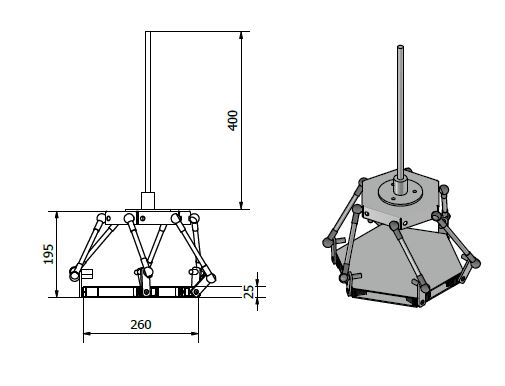
\includegraphics[width=0.8\linewidth]{Figures/Assembly}
	\caption[Assembled Platform]{Assembly of Stewart Platform}
	\end{figure}
\end{center}
\begin{center}
	\begin{figure}[!h]
	\centering
	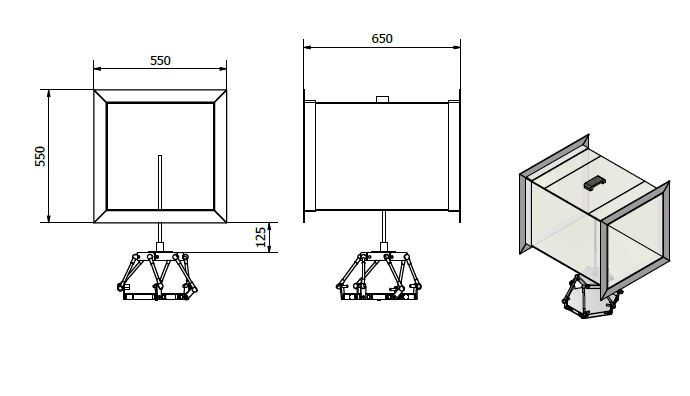
\includegraphics[width=0.8\linewidth]{Figures/Test-section}
	\caption[Model placement in Test Section]{Stewart platform and Test section configuration}
	\end{figure}
\end{center}
\clearpage
\subsection{Stewart Platform Simulation}
Stewart Platform simulation was done on MatLab using the Inverse kinematics equations. Different servo angles for different platform movements can be obtained from the simulation. The angles for yaw, pitch and roll could be adjusted during simulations to predict the maximum allowable angle values. Value of displacement in the x-, y- and z-directions could also be adjusted enabling us to predict the maximum allowable displacement in the respective directions.
\begin{center}
	\begin{figure}[!h]
	\centering
	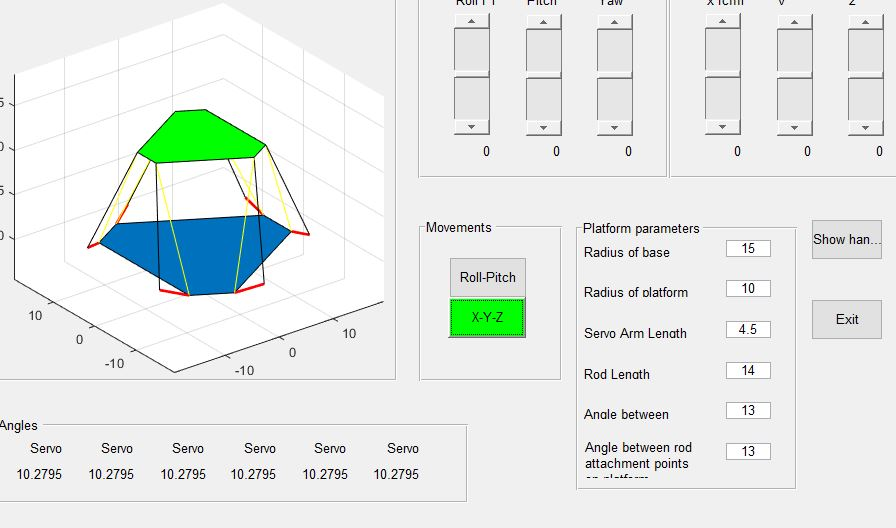
\includegraphics[width=0.75\linewidth]{Figures/Matlab}
	\caption[Linear displacements]{Matlab simulation for x-y-z movements}
	\end{figure}
\end{center}
\begin{center}
	\begin{figure}[!htb]
	\centering
	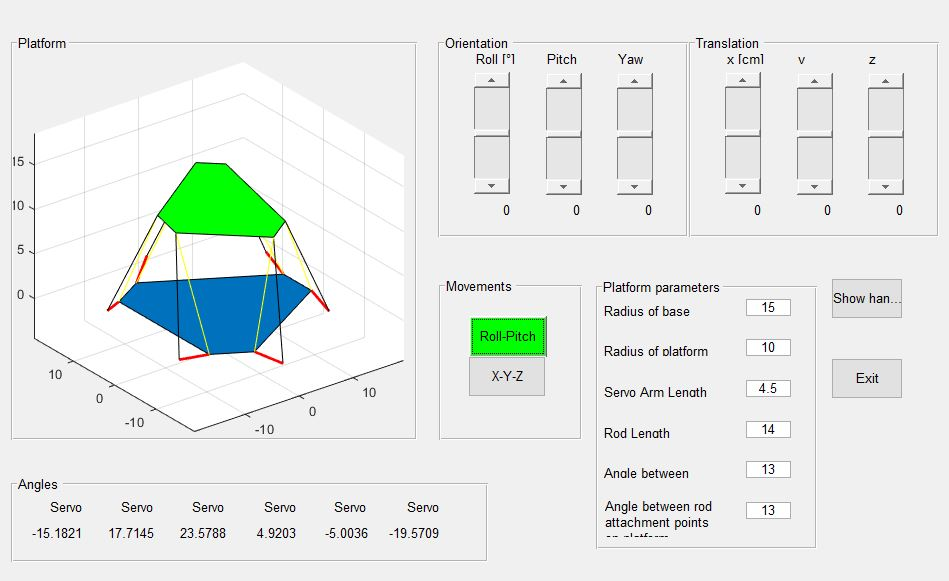
\includegraphics[width=0.75\linewidth]{Figures/Matlab2}
	\caption[Angular displacements]{Matlab simulation for yaw,pitch and roll movements}
	\end{figure}
\end{center}
\subsection{Finite Element Analysis on Stewart Platform}
Finite Element Analysis was done on FEA environment in Autodesk inventor. A maximum possible model weight of 50N was applied on the platform. 
A ststic analysis test was performed and the following results were obtained:
\begin{center}
	\begin{figure}[!htb]
	\centering
	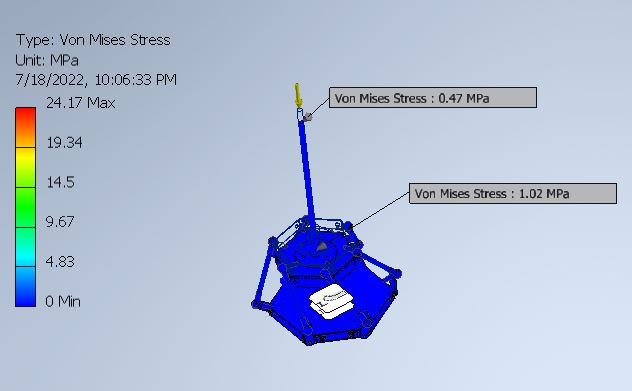
\includegraphics[width=0.75\linewidth]{Figures/Von}
	\caption[Von Mise's Stress]{Von Mise's Stress}
	\end{figure}
\end{center}
\begin{table}[!h]
\caption{FEA Results}
\end{table}
\begin{center}
\begin{tabular}{|l|l|l|}
\hline
\textbf{Name} & \textbf{Minimum} & \textbf{Maximum}\\
\hline
Von Mise's & 0 MPa & 24.1718 MPa\\
\hline
Displacement & 0 mm & 23.7377 mm\\
\hline
Safety Factor & 10.3426 ul & 15 ul\\
\hline
Equivalent Strain & 0 ul & 0.000153819 ul\\
\hline
\end{tabular}
\end{center}
Von Mise's stress does not exceed the Yield Stress of Aluminum (275 MPa) hence the platform will not yield under this applied load.

Application of loads on the platform translates to induced strain in the Stewart platform legs. This will provide an input for the strain gauges used for force measurements.

\section{Human Machine Interface}
The user interface of the platform was programmed using golang and this resulted in the view below with the use of sliders for platform positioning and buttons to set model orientationa and start data collection.
\begin{center}
	\begin{figure}[!h]
	\centering
	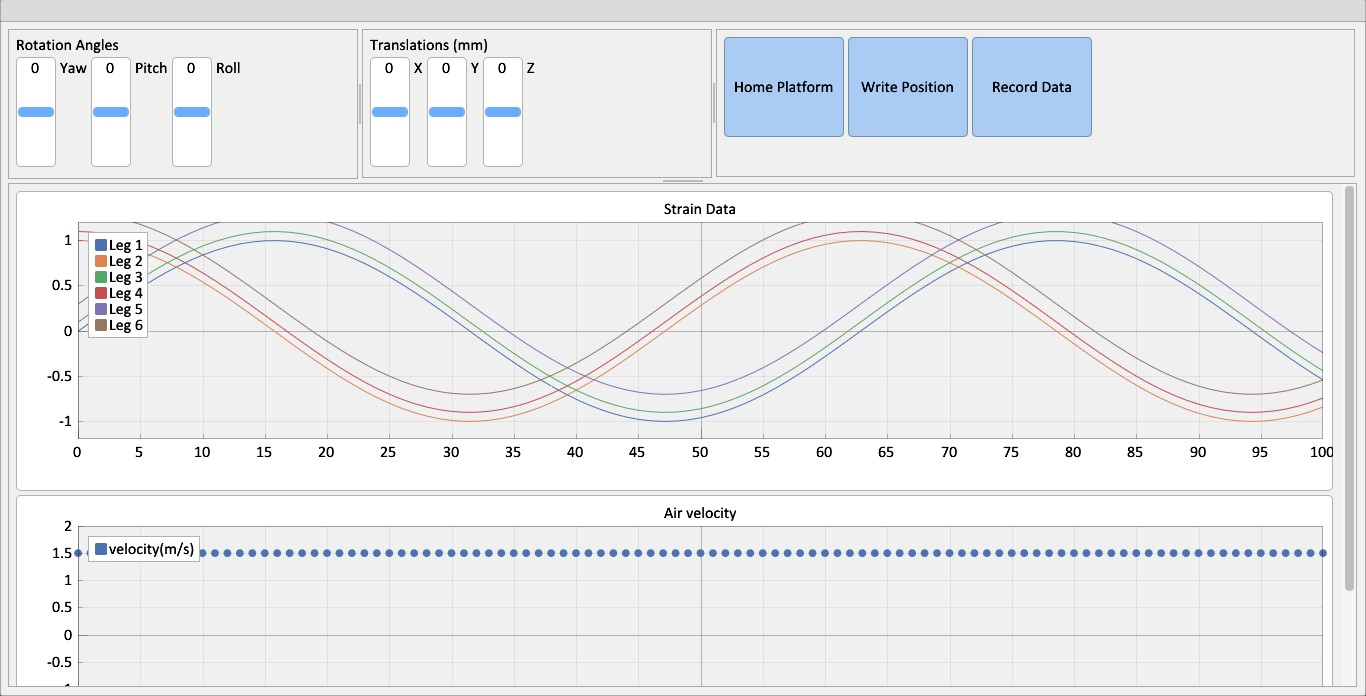
\includegraphics[width=0.7\linewidth]{Figures/hmi}
	\caption[HMI Dashboard]{HMI Dashboard}
	\end{figure}
\end{center}

\section{PCB}
The schematics from the electrical designs as seen in the aooendix were routed to generate a PCB ready for maufucture. This is shown in the 3D rennder below:
\begin{center}
	\begin{figure}[!h]
	\centering
	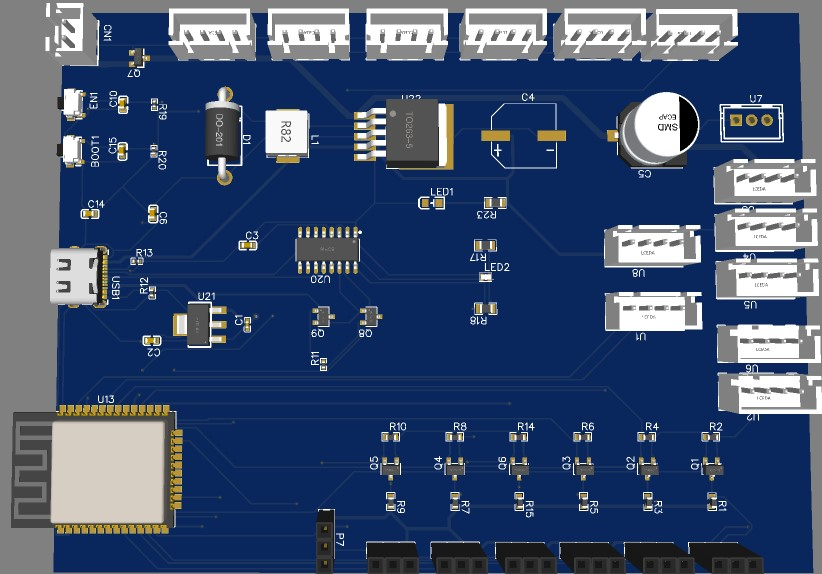
\includegraphics[width=0.7\linewidth]{Figures/pcb}
	\caption[HMI Dashboard]{HMI Dashboard}
	\end{figure}
\end{center}
